\subsection{External Interface Requirements}
	\subsubsection{User Interfaces}
		Here we provide some mockups to show how the interface should appear to the user:\newline
		
		\begin{figure}[H]	
			\centerline{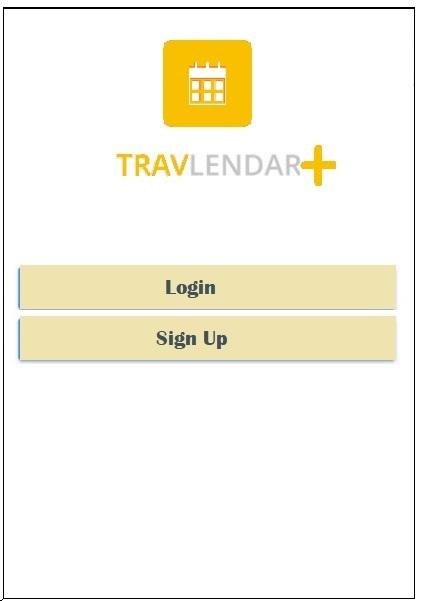
\includegraphics[scale=0.4]{Images/Login}}
			\caption{Login}
		\end{figure}	
		\begin{figure}[H]		
			\centerline{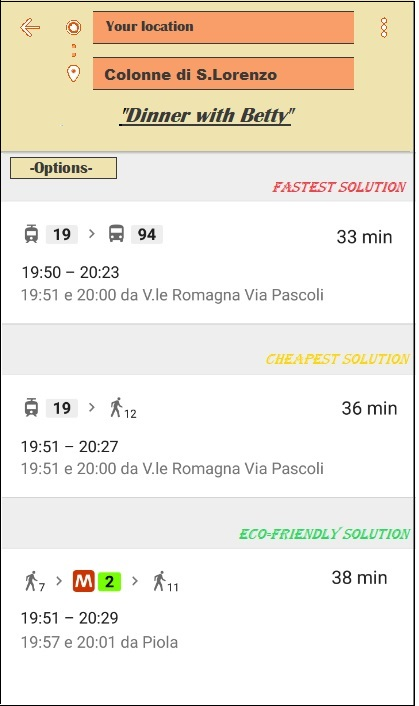
\includegraphics[scale=0.4]{Images/suggestedsolution}}
			\caption{Select solution}
		\end{figure}	
		\begin{figure}[H]
			\centerline{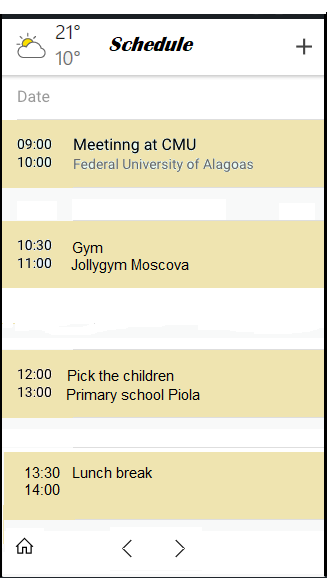
\includegraphics[scale=0.4]{Images/schedule}}
			\caption{Visualize schedule}
		\end{figure}
	
	\subsubsection{Hardware Interfaces}
	\subsubsection{Software Interfaces}
	\subsubsection{Communication Interfaces}
\subsection{UML modeling}
	\subsubsection{Use Case diagram}
		\textbf{Diagram} \\
		\indent\textit{TODO: here an image will be attached}
		\newline
		\renewcommand{\arraystretch}{1.6} % increase line height
		
		\medskip %leave a bit of space before the next 'section'
		\vbox{ % to avoid page breaking
			\noindent
			\textbf{User creates event}
			\medskip\\
			\begin{tabu} to \textwidth {| X[\fcWidth,r,p] | X[1-\fcWidth,l,p] |}
				\hline\textbf{Use case:} & User creates an event
				\\
				\hline\textbf{Actors:} & User
				\\
				\hline\textbf{Entry condition:} & The user must be logged
				\\
				\hline\textbf{Flow of events:} & The user creates an event (a meeting, appointment or generic event) giving it a name;\newline
				User specifies the location of the event;\newline
				User specifies details such as passengers or baggage;\newline
				User selects a travel mean taking to account app’s suggestion;\newline
				The app takes note of the settings and send a confirmation;\newline
				The app redirects the user to the main page.
				\\
				\hline\textbf{Secondary flows:} & User does not specify a travel mean and let it blank;\newline
				The app takes anyway note of the setting and alert the user of the missing information; \newline
				The app redirects the user to the main page.
				\\
				\hline\textbf{Exceptions:} & Warnings messages are created in the following cases:
				\begin{itemize}
					\item User creates an event that overlaps another event;
					\item User creates an event with a location that is unreachable in the allocated time;
					\item User creates an event that violates the set constraints about the break windows.
				\end{itemize}
				\\
				\hline\textbf{Post conditions:} & The user is successfully redirected to the main page.
				\\
				\hline
			\end{tabu}
			\bigskip %leave a bit of space after the table
		}
		
		\vbox{ % to avoid page breaking
			\noindent
			\textbf{Sign Up}
			\medskip\\
			\begin{tabu} to \textwidth {| X[\fcWidth,r,p] | X[1-\fcWidth,l,p] |}
				\hline\textbf{Use case:} & Sign Up
				\\
				\hline\textbf{Actors:} & Person
				\\
				\hline\textbf{Entry condition:} &user must be not already logged;
				\\
				\hline\textbf{Flow of events:} & the person inserts full name and email contact;\newline
				the app send an email with the confirmation link;\newline
				the person give the confirmation trough the link on the mail;\newline
				the app give the welcome to the new user.
				
				\\
				\hline\textbf{Secondary flows:} & none.
				\\
				\hline\textbf{Exceptions:} &the person inserts a wrong email contact;\newline
				the sign up cannot proceed.
				
				\\
				\hline\textbf{Post conditions:} & the person is successfully signed up and become an actual logged user.
				\\
				\hline
			\end{tabu}
			\bigskip %leave a bit of space after the table
		}
		
		\vbox{ % to avoid page breaking
			\noindent
			\textbf{Initial settings configuration}
			\medskip\\
			\begin{tabu} to \textwidth {| X[\fcWidth,r,p] | X[1-\fcWidth,l,p] |}
				\hline\textbf{Use case:} & Initial settings configuration
				\\
				\hline\textbf{Actors:} & User
				\\
				\hline\textbf{Entry condition:} & the User just has just completed the sign up process;\newline
				user must be logged.
				
				\\
				\hline\textbf{Flow of events:} & User insert sequentially the following  information:
				\begin{itemize}
				\item 	Credit card;
				\item 	Driving licence;
				\item 	Break time windows;
				\item	Interest for Eco-friendly solutions on the travel means.
				\item	Constraints on travel means.
				\end{itemize}
				The app, for each step,  check the info and send a confirmation;
				The app redirects the user to the main page.
				
				\\
				\hline\textbf{Secondary flows:} & User skips to specify one or more information that could be specified later in the settings.\newline
				The app notifies the user about the missing information and redirects anyway the user to the main page.
				
				\\
				\hline\textbf{Exceptions:} & user inserts inconsistent information (incorrect credid-card/licence information, break time shorter than 30 minutes);\newline
				The app allerts the user and asks him to insert again the info.
				\\
				\hline\textbf{Post conditions:} & the set configurations are successfully saved and the user is redirected to the main page.
				\\
				\hline
			\end{tabu}
			\bigskip %leave a bit of space after the table
		}
		
		\vbox{ % to avoid page breaking
			\noindent
			\textbf{User visualizes the appointment}
			\medskip\\
			\begin{tabu} to \textwidth {| X[\fcWidth,r,p] | X[1-\fcWidth,l,p] |}
				\hline\textbf{Use case:} & User visualizes the appointment.
				\\
				\hline\textbf{Actors:} & User
				\\
				\hline\textbf{Entry condition:} & user must be logged;\newline
				the event must exist;
				
				\\
				\hline\textbf{Description:} & user visualize an appointment and eventually:
				\begin{itemize}
					\item If not specified yet, set a travel mean;
					\item Modify the previous travel mean or other detail such as location, baggage or passengers;
					\item Buy a ticket for the travel mean;
					\item Rent a shared vehicle if is the proper time to do that and locate the nearest one;
					\item Delete the appointment. 
				\end{itemize}\\
				\hline
			\end{tabu}\\
			\bigskip %leave a bit of space after the table
		}
		
		\vbox{ % to avoid page breaking
			\noindent
			\textbf{User buy travel ticket}
			\medskip\\
			\begin{tabu} to \textwidth {| X[\fcWidth,r,p] | X[1-\fcWidth,l,p] |}
				\hline\textbf{Use case:} & User buy travel ticket
				\\
				\hline\textbf{Actors:} & User
				\\
				\hline\textbf{Entry condition:} & user must be logged; \newline
				user must have added a payment card .
				
				\\
				\hline\textbf{Flow of events:} &User select an event;\newline
				User,  through the app, searches for tickets for the specified travel mean; \newline
				User select the ticket’s option and picks one;\newline
				User proceeds with the payment;\newline
				The payment operation ends successfully;\newline
				The app send a confirmation and redirects the user to the main page;
				
				\\
				\hline\textbf{Secondary flows:} & none
				\\
				\hline\textbf{Exceptions:} & The payment is rejected (not enough credit, expired card, ..);\newline
				The app notifies the user; \newline
				The app redirect the user to the home page;
				
				\\
				\hline\textbf{Post conditions:} & User successfully books the tickets and is redirected to the main page.
				\\
				\hline
			\end{tabu}
		}
	\subsubsection{Class diagram}
		% don't really know what happens here, but it is fine graphically
		% ((I'm referring to '\paperwidth-1')
		\begin{figure}[H]
			\centerline{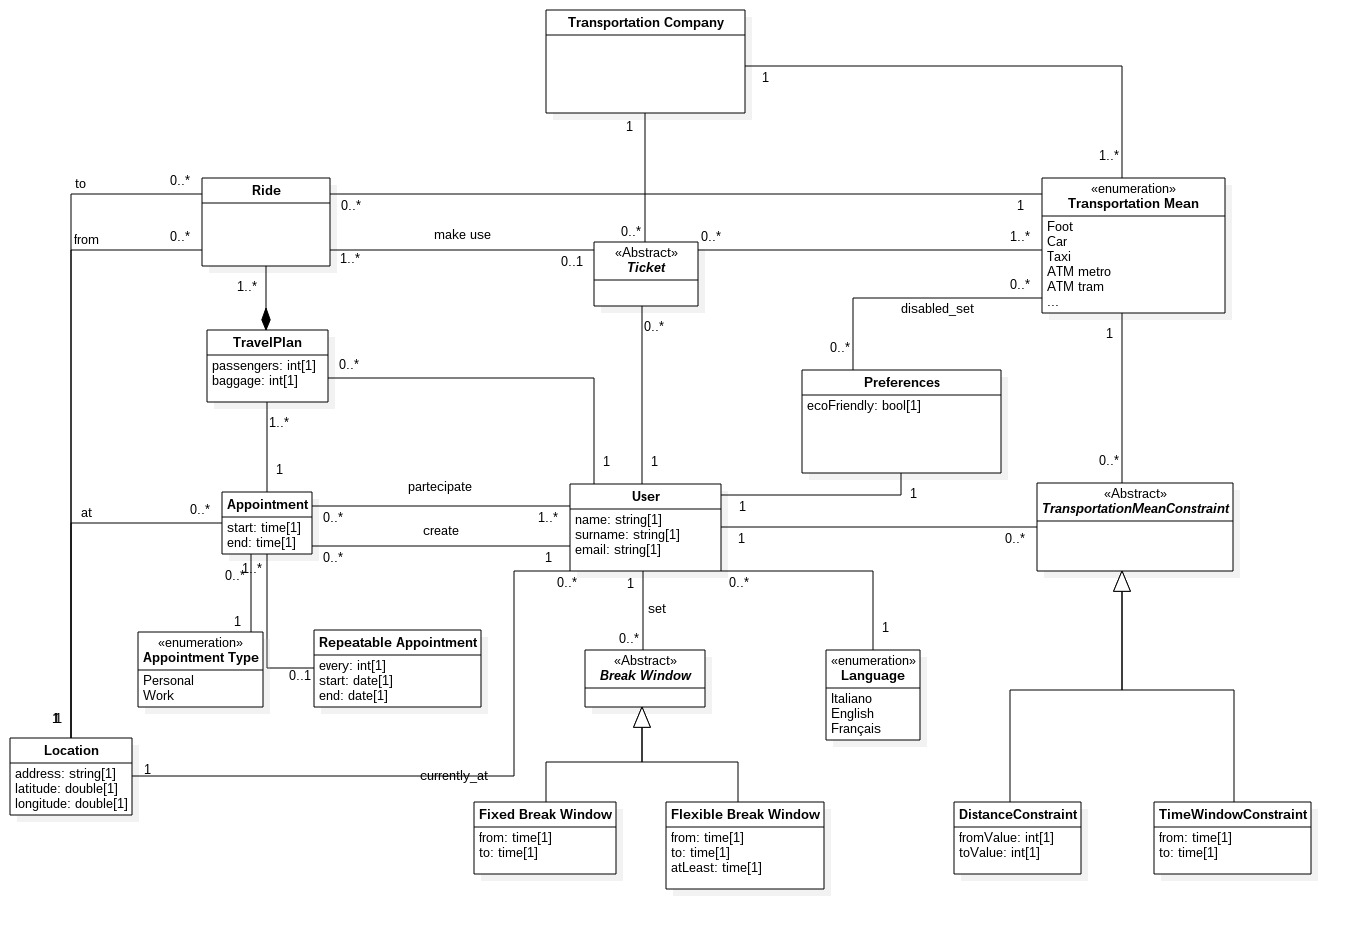
\includegraphics[width=\paperwidth-1]{Images/ClassDiagram}}
			\caption{General class diagram}
		\end{figure}
	\subsubsection{Activity diagrams}
		\begin{figure}[H]
			\centerline{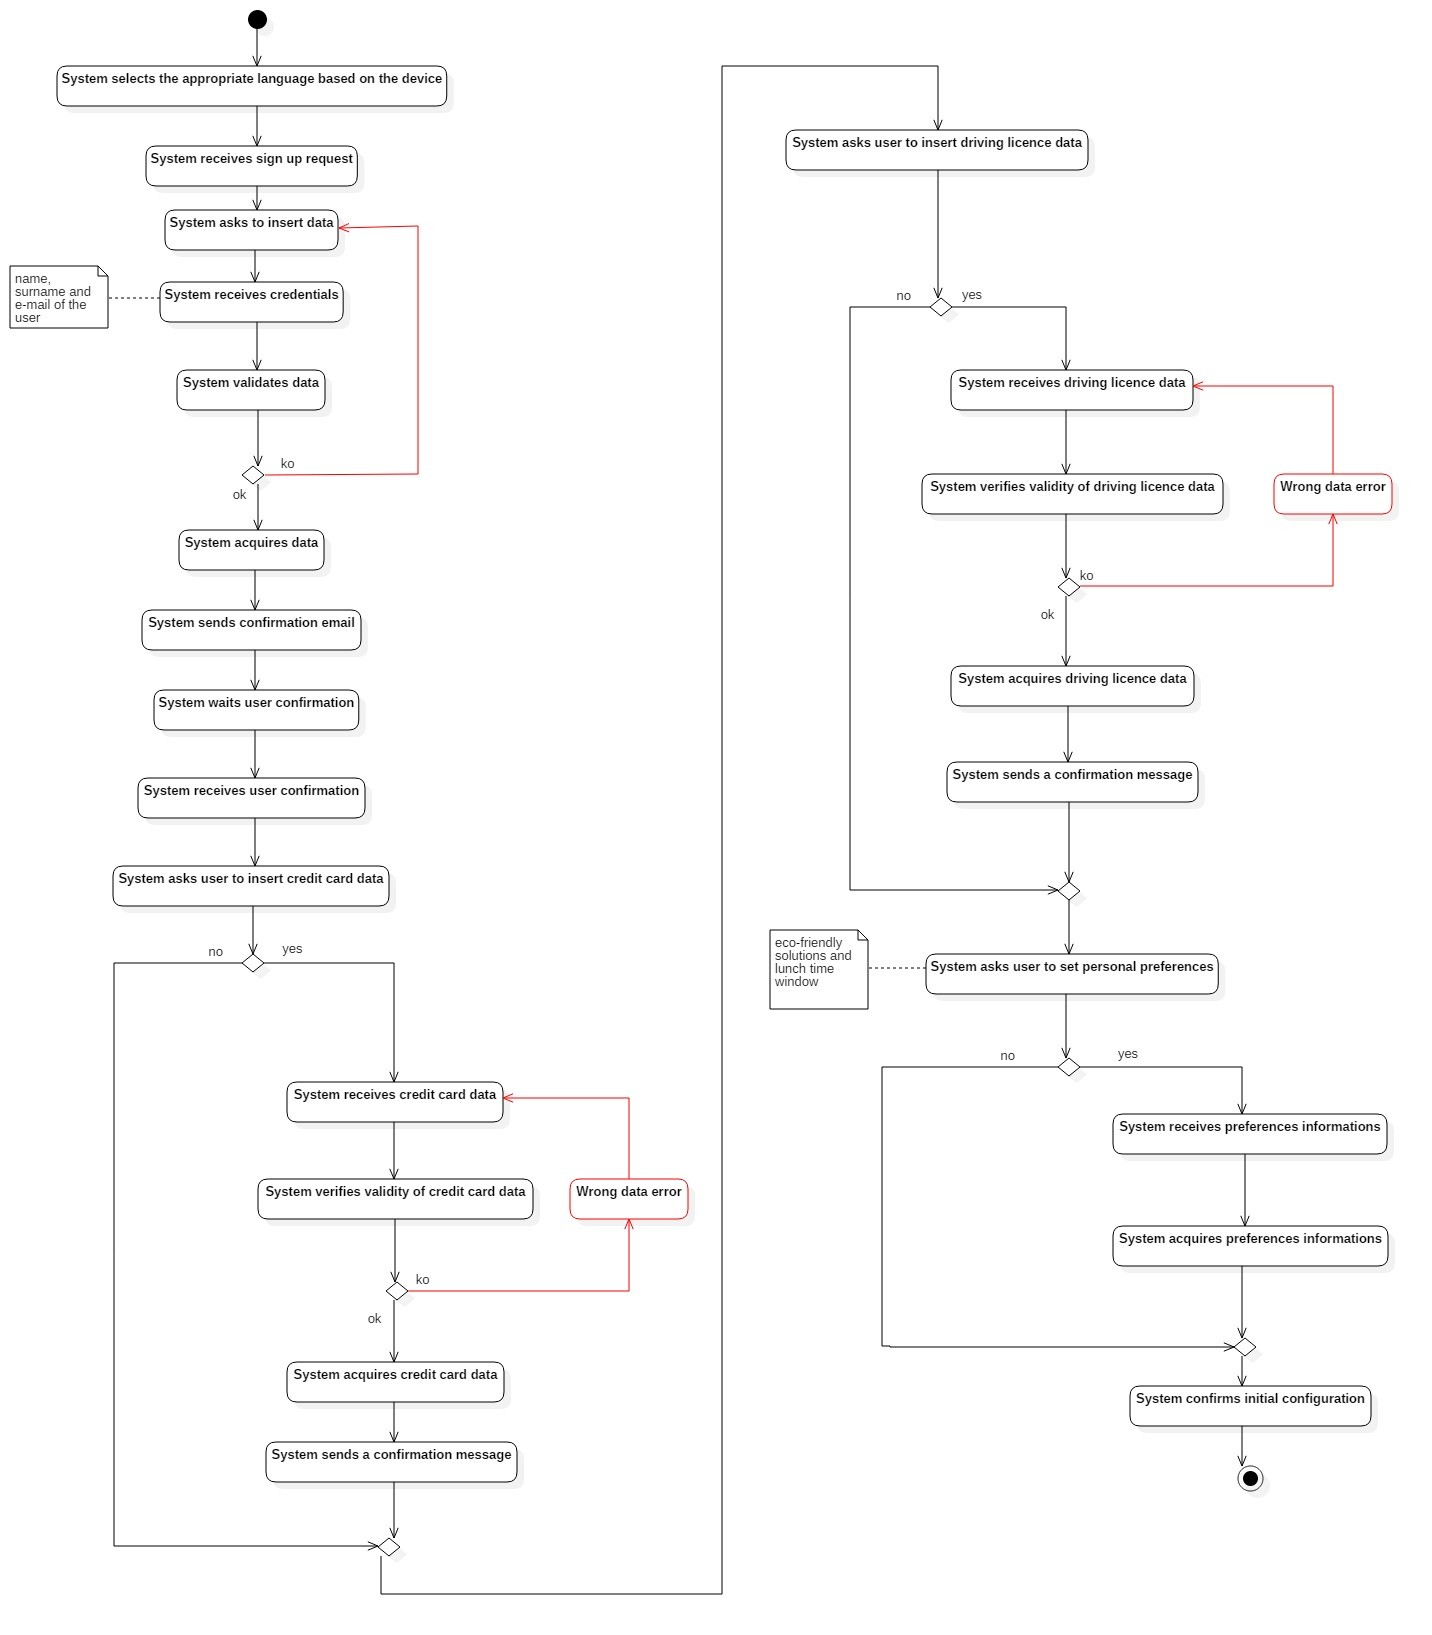
\includegraphics[height=0.75\paperheight]{Images/RegistrationDiagram}}
			\caption{Registration diagram}
		\end{figure}

%		\begin{figure}[H]
%			\centerline{\includegraphics[width=\paperwidth-1]{Images/AppointmentCreationDiagram}}
%			\caption{Appointment creation diagram}
%		\end{figure}
\subsection{Functional Requirements}
\subsection{Performance Requirements}
\subsection{Design Constraints}
	\subsubsection{Standard compliance}
	\subsubsection{Hardware limitations}
	\subsubsection{Any other constraint}
\subsection{Software System Attributes} 
	\subsubsection{Reliability}
	\subsubsection{Availability}
	\subsubsection{Security}
	\subsubsection{Maintainability}
	\subsubsection{Portability}